\documentclass[10pt,a4paper]{article}
\usepackage[spanish,activeacute]{babel}
\usepackage[utf8]{inputenc}
\usepackage{amsmath}
\usepackage{blindtext}
\title{Este es un titulo}
\author{Fernando Sosa Torres}
\usepackage{graphicx}

\usepackage{float}
\graphicspath{{images/}}
\begin{document}
\maketitle
\part{part dice ahi}
\section{Introduccion} 
hola amigos de nuevo
\blindtext

hola amigos

adios amigos
\section{Resultados Los buenos}
Tenemos la informacion de la seccion
\section{Resultados}
lorem lorem

Tenemos una \textbf{oracion} con la personalizacion que nosotros \textit{deseamos}
\subsection{''subsection''}

\begin{enumerate}
	\item Papas
	\item Leche
	\item frijoles
	\item Tenemos otro elemento
\end{enumerate}
\begin{itemize}
	\item papas
	\item papel
	\item Hamburguesas
	\item comida mascotas
	\begin{itemize}
		\item comida para gato
		\item carne
		\item agregando otra carne
	\end{itemize}
\end{itemize}

\begin{figure}[H]
\centering
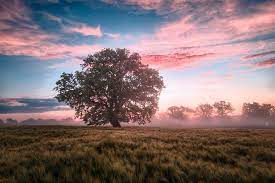
\includegraphics[width=0.5\textwidth]{imagen}
\caption{El paisaje de como nosotros hablamos}
\label{paisaje}
\end{figure}

Haciendo referencia a la imagen de la imagen \ref{paisaje} 

lsdkjflsadkjf

colocando texto a una expresion matematica  $x^2$
colcoando otra expreision matematica $\sum_2^\infty$

\begin{equation}
	\sum_2^\infty x = \infty
\end{equation}


\begin{gather}
	\frac{x}{2} = 4\\
	\implies x = 6
\end{gather}{}


\begin{tabular}{| c | c |}
\hline
Fruta & Cantidad \\ \hline
Manzana & 4 \\
\hline
Naranja & 10 \\
\hline
Plátano & 3 \\ \hline
\end{tabular}


\end{document}
